\documentclass{beamer}
\usepackage{graphicx}

\setbeamertemplate{footline}[frame number]

\begin{document}

\begin{frame}
\frametitle{Batches of Local Modifications}
\begin{columns}[T]
\begin{column}{.5\textwidth}
\begin{itemize}
\item Choose a large set of operations to do simultaneously
\item Cannot overlap, hence independent set
\item ``Maximal" : cannot add more without overlap
\item Try to select ``best" operations ?
\end{itemize}
\end{column}
\begin{column}{.5\textwidth}
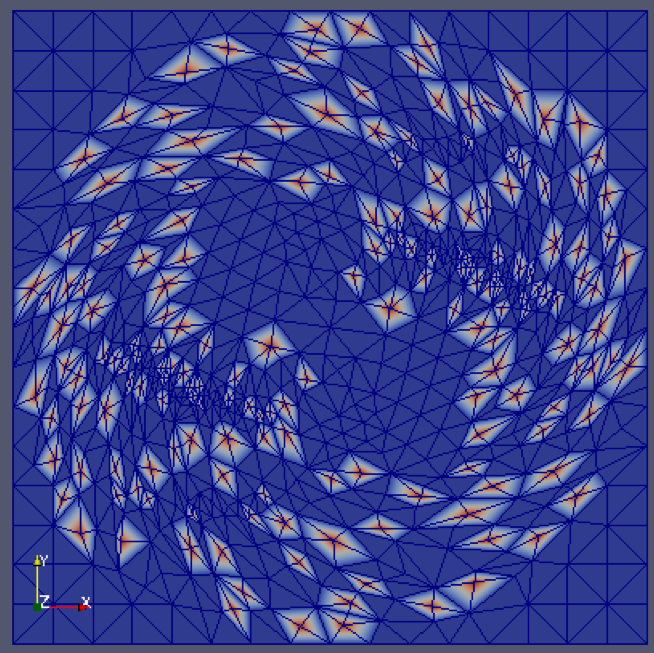
\includegraphics[width=\textwidth]{coarsen_indset.png}
\end{column}
\end{columns}
\end{frame}

\begin{frame}
\frametitle{Adjacency Graph Structure}
\begin{columns}[T]
\begin{column}{.5\textwidth}
\begin{itemize}
\item Maps from one dimension to another
\item Adjacency list for one entity is contiguous
\item Offsets array indicates start/end of each sub-list
\item Example usage: upward (vertices to elements) adjacency
\end{itemize}
\end{column}
\begin{column}{.5\textwidth}
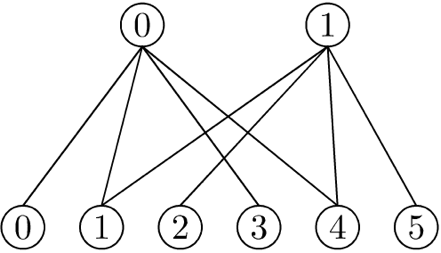
\includegraphics[width=.8\textwidth]{graph.png}
\vspace{1.5cm}
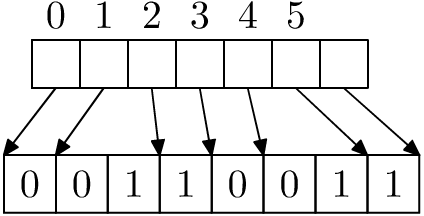
\includegraphics[width=.8\textwidth]{offsets.png}
\end{column}
\end{columns}
\end{frame}

\begin{frame}
\frametitle{Derivation and Caching}
\begin{columns}[T]
\begin{column}{.5\textwidth}
\begin{itemize}
\item Always start with down-to-vertex adjacency
\item Compute other adjacencies when requested
\item Frequent repeated requests
\item High cost of computation
\begin{itemize}
\item 50\% of adapt time !
\end{itemize}
\item Good use case for caching
\item Tradeoff with memory usage ?
\end{itemize}
\end{column}
\begin{column}{.5\textwidth}
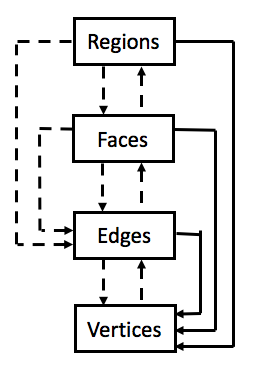
\includegraphics[width=.8\textwidth]{adjs.png}
\end{column}
\end{columns}
\end{frame}

\begin{frame}
\frametitle{Batched Array Modifications}
\begin{columns}[T]
\begin{column}{.5\textwidth}
\begin{enumerate}
\item Start with old mesh
\item Evaluate all possible operations (of one kind)
\item Choose independent set based on best quality
\item Apply entire set using \texttt{parallel\_for}, one cavity per iteration
\end{enumerate}
\end{column}
\begin{column}{.5\textwidth}
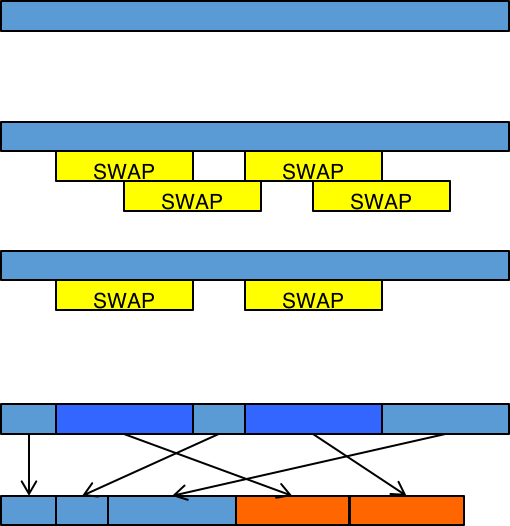
\includegraphics[width=\textwidth]{batch_steps.png}
\end{column}
\end{columns}
\end{frame}

\end{document}
